\subsection{Absorci�n}
\begin{frame}
\frametitle{}

\begin{figure}
\begin{tikzpicture}[node distance=0.5cm, auto,>=latex', thick]
\scriptsize
    % We need to set at bounding box first. Otherwise the diagram
    % will change position for each frame.
    \path[use as bounding box] (-1.5,0) rectangle (12,-2);

    % TT methodology     
    \node [phase]                        (monitoreo)     {Vigilancia};
    \node [phase, below of=monitoreo]    (choice)        {Elecci�n};
    \node [phase, below of=choice]       (acquisition)   {Adquisici�n};
    \node [phase, below of=acquisition]  (adaptation)    {Adaptaci�n};
    \node [phase2,below of=adaptation]   (absortion)     {Absorci�n};
    \node [phase, below of=absortion]    (aplication)    {Aplicaci�n};
    \node [phase, below of=aplication]   (difusion)      {Difusi�n};

    %%%%%%%%%%%%%%%%%%%%%%%%%%%%%%%%%%%%%%%%%%%%&
    %            Absorci�n
    %%%%%%%%%%%%%%%%%%%%%%%%%%%%%%%%%%%%%%%%%%%%&
    \onslide<1> \node [ph_explain, right=.5cm of adaptation.east] (exp_absortion)     
    {
      \begin{center} \textbf{Absorci�n} \end{center}
    \begin{itemize}
     \item Absorci�n: Capacidad del receptor para absorber, asimilar y utilizar la tecnolog�a.

     \item Se deben generar habilidades t�cnicas y humanas para operar y cambiar la nueva tecnolog�a

      \begin{itemize}
        \scriptsize
        \item Banco de proyectos.
        \item  Metodolog�as de dise�o y procesos de fabricaci�n.
   \end{itemize}
    \end{itemize}
    };

    \onslide<2> \node [ph_explain2, right=.5cm of adaptation.east] (exp_adaptation)    
    {
      \begin{center} \textbf{Plataforma ECB\_ARM7 } \end{center}
        \centering
          \mbox{
            \subfigure{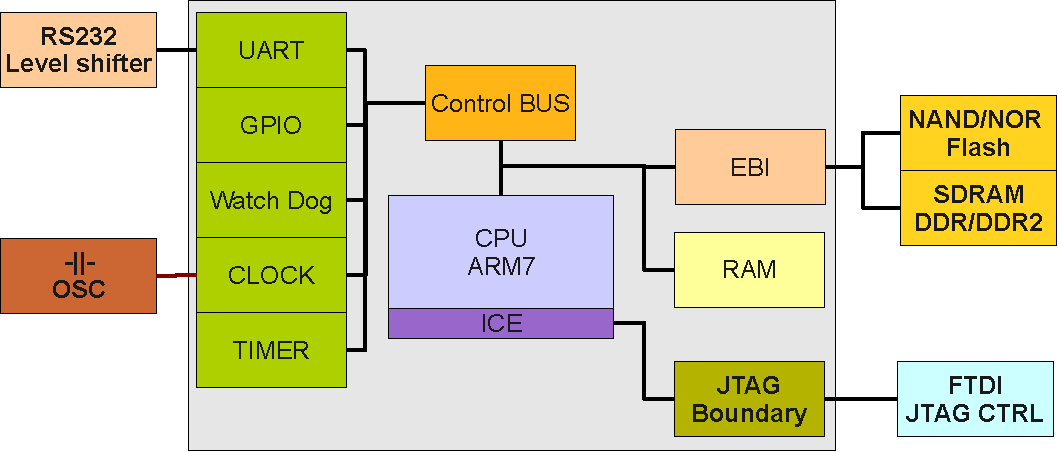
\includegraphics[scale=.32]{../images/ECB_ARM7_Block.pdf}}
            \subfigure{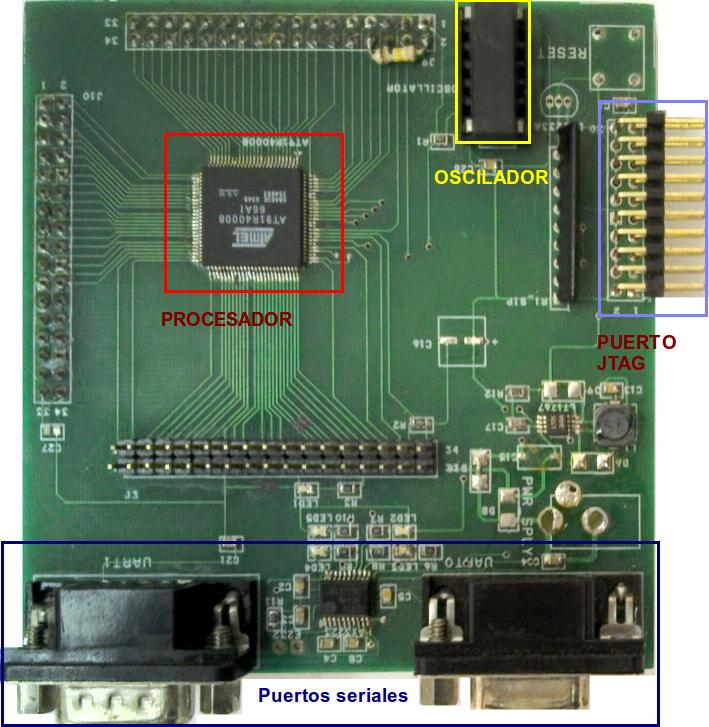
\includegraphics[scale=.15]{../images/ECB_ARM7.jpg}}
          }
        \resizebox{!}{.4cm}{
            \footnotesize
            \begin{tabular}{|l|l|l|l|}
              \hline
              \textbf{CPU}  & \textbf{Capas} & \textbf{Montaje}  &\textbf{OS}
              \\ \hline
              ARM7,33M     & 2              & local Manual.     & eCos 
              \\ \hline 
            \end{tabular}
        }
    };

    \onslide<3> \node [ph_explain2, right=.5cm of adaptation.east] (exp_adaptation)    
    {
      \begin{center} \textbf{Plataforma Xport } \end{center}
      \centering
        \mbox{
          \subfigure{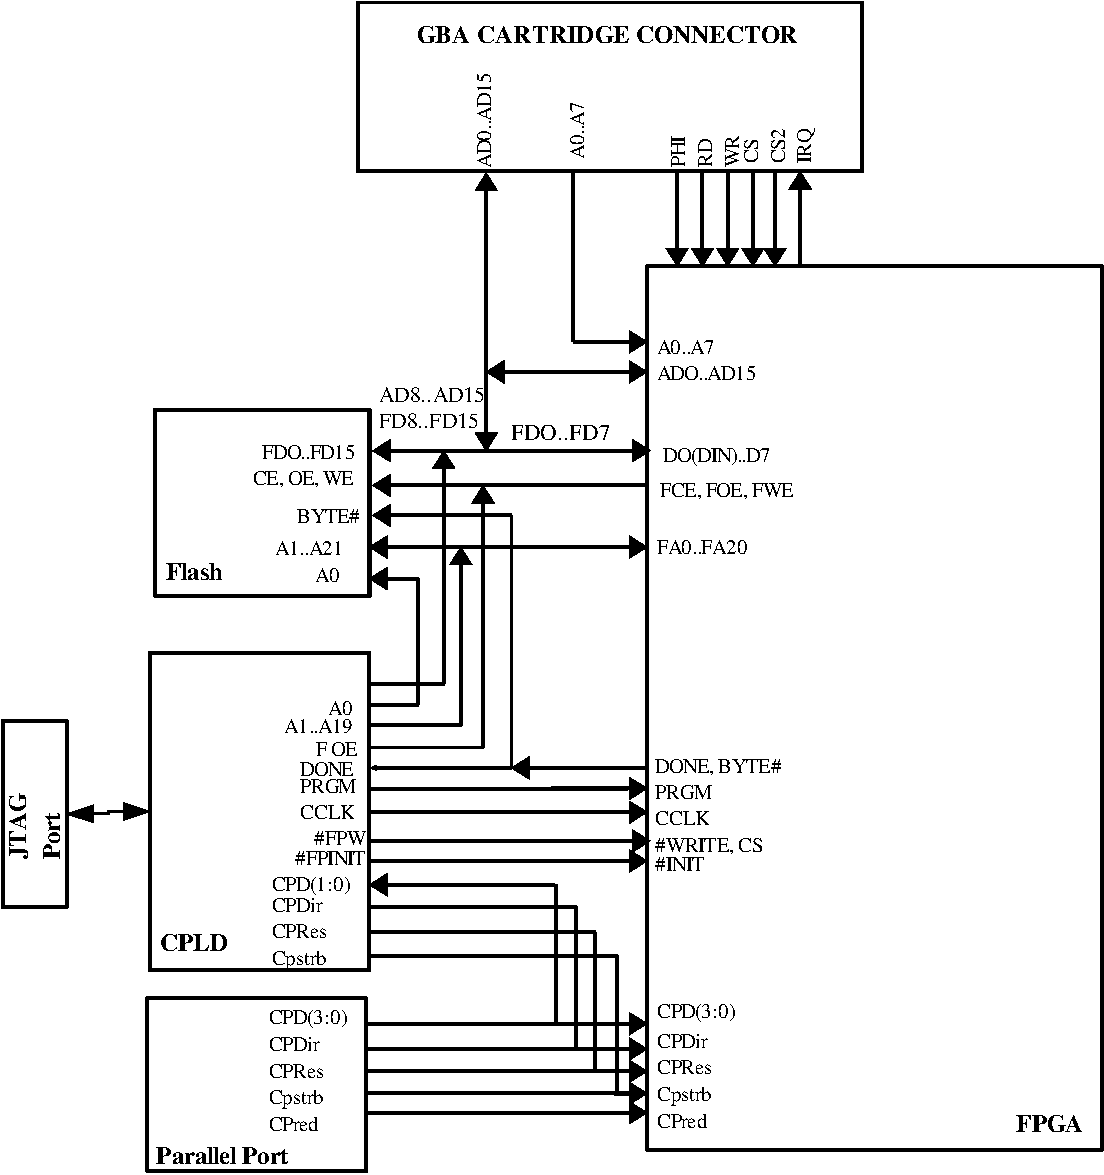
\includegraphics[scale=.28]{../images/xport_Block.pdf}}
          \subfigure{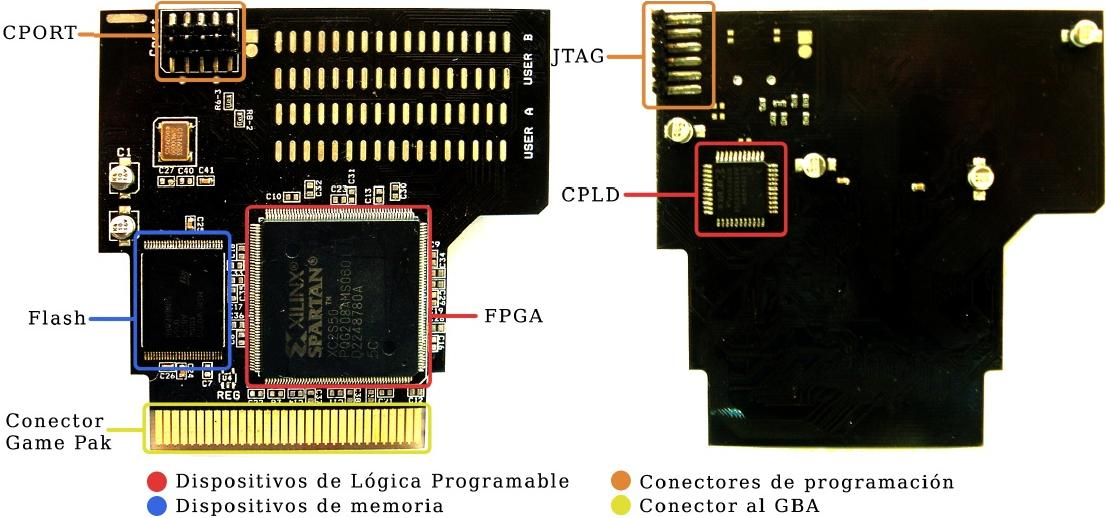
\includegraphics[scale=.2, angle=90]{../images/xport.jpg}}
        }
        \resizebox{!}{.4cm}{
            \footnotesize
            \begin{tabular}{|l|l|l|l|}
              \hline
              \textbf{CPU}  & \textbf{Capas} & \textbf{Montaje}  &\textbf{OS}
              \\ \hline
              ARM7,50M     &    2           & local Manual.     & eCos
              \\ \hline 
            \end{tabular}
        }
     };
 
    \onslide<4> \node [ph_explain2, right=.5cm of adaptation.east] (exp_adaptation)    
    {
      \begin{center} \textbf{Plataforma ECB\_AT91\_V1} \end{center}
      \centering
      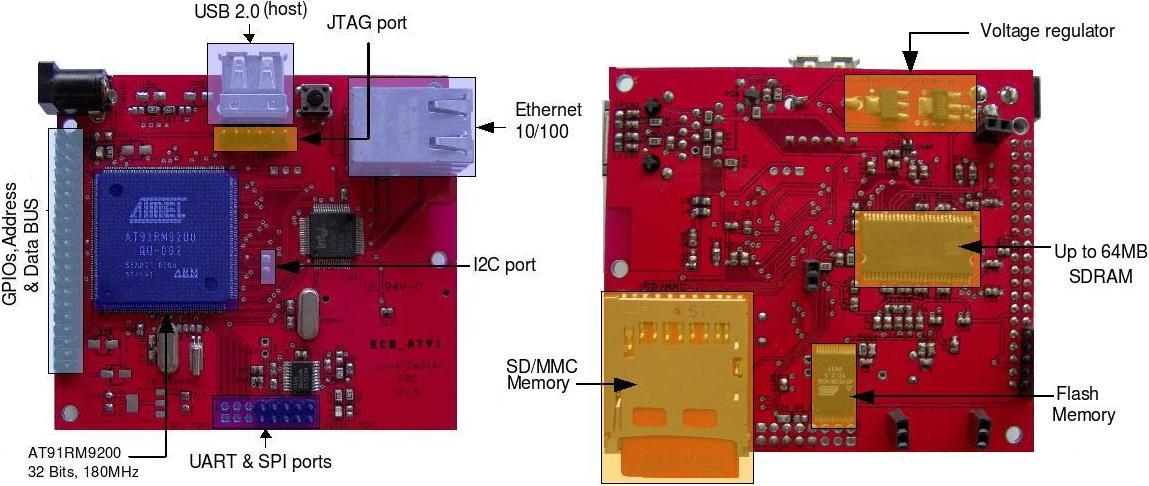
\includegraphics[scale=.3]{../images/ECB_AT91_V1.jpg}
      \\
        \resizebox{!}{.4cm}{
            \footnotesize
            \begin{tabular}{|l|l|l|l|}
              \hline
              \textbf{CPU}  & \textbf{Capas} & \textbf{Montaje}  &\textbf{OS}
              \\ \hline
              ARM920,180M   &    2           & local Manual/Autom. & 100
              \\ \hline 
            \end{tabular}
        }
    };

    \onslide<5> \node [ph_explain2, right=.5cm of adaptation.east] (exp_adaptation)    
    {
      \begin{center} \textbf{Plataforma ECB\_AT91\_V2} \end{center}
        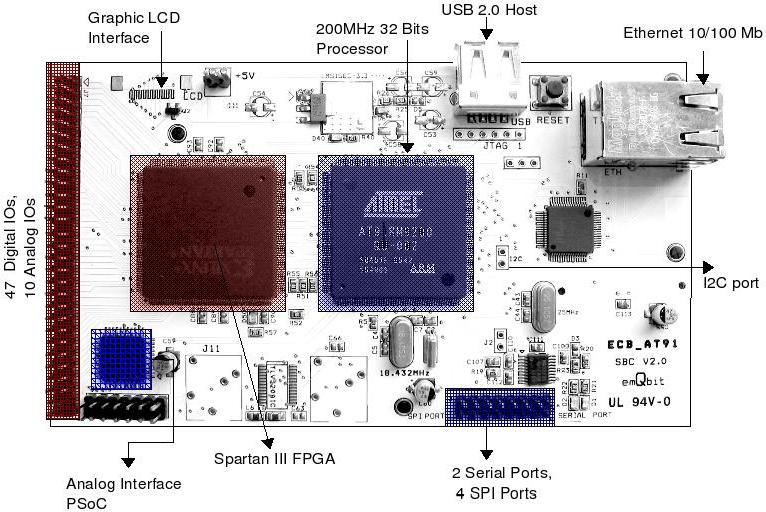
\includegraphics[scale=.43]{../images/ECB_AT91_V2.jpg}
        \\
        \resizebox{!}{.4cm}{
            \footnotesize
            \begin{tabular}{|l|l|l|l|}
              \hline
              \textbf{CPU}  & \textbf{Capas} & \textbf{Montaje}  &\textbf{OS}
              \\ \hline
              ARM920 180M   &     4          & local Manual.     & Linux 
              \\ \hline 
            \end{tabular}
        }
    };
 
    \onslide<6> \node [ph_explain2, right=.5cm of adaptation.east] (exp_adaptation)    
    {
      \begin{center} \textbf{Plataforma ECBOT} \end{center}
      \centering
       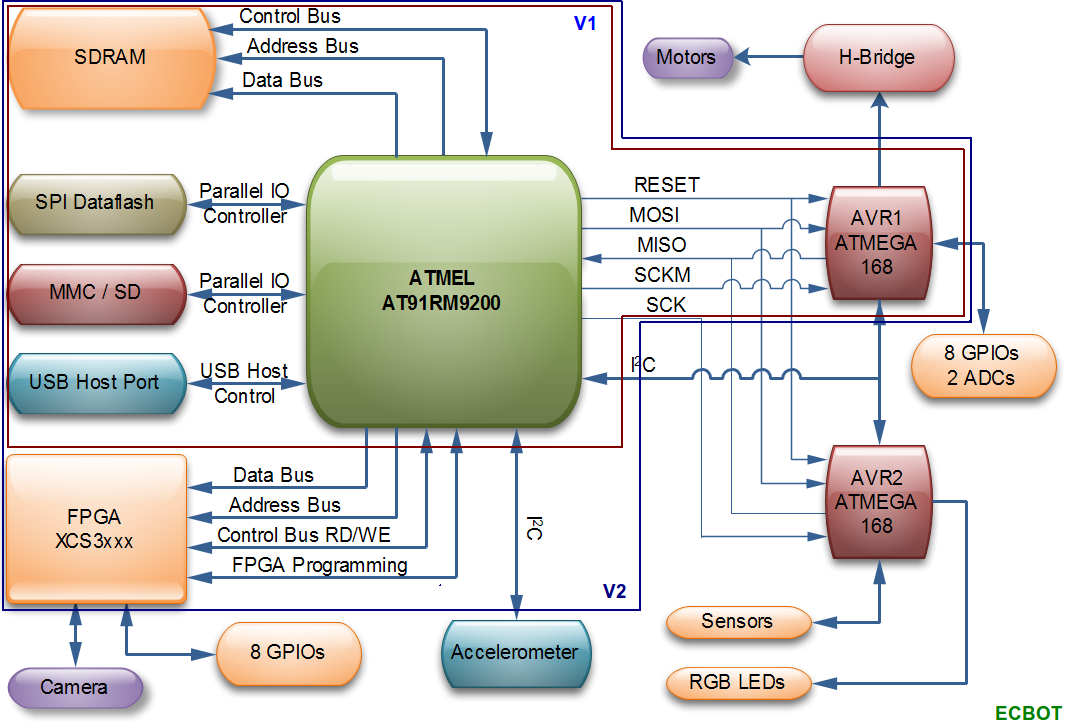
\includegraphics[scale=.3]{../images/ECBOT_Block.png} \\
       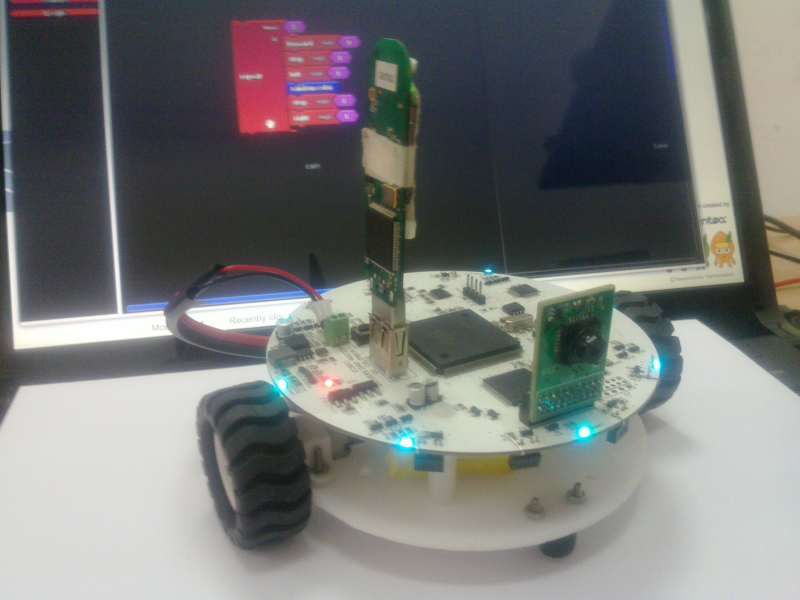
\includegraphics[scale=.15]{../images/ECBOT.png}  
       \\
       \resizebox{!}{.35cm}{
          \footnotesize
          \begin{tabular}{|l|l|l|l|}
            \hline
            \textbf{CPU}  & \textbf{Capas} & \textbf{Montaje}  &\textbf{OS}
            \\ \hline
            ARM920 180M   &       4        & local Manual.     & Linux
            \\ \hline 
          \end{tabular}
        }
    };

    \onslide<7> \node [ph_explain2, right=.5cm of adaptation.east] (exp_adaptation)    
    {
      \begin{center} \textbf{Plataforma ECB\_BF532} \end{center}
     \centering
       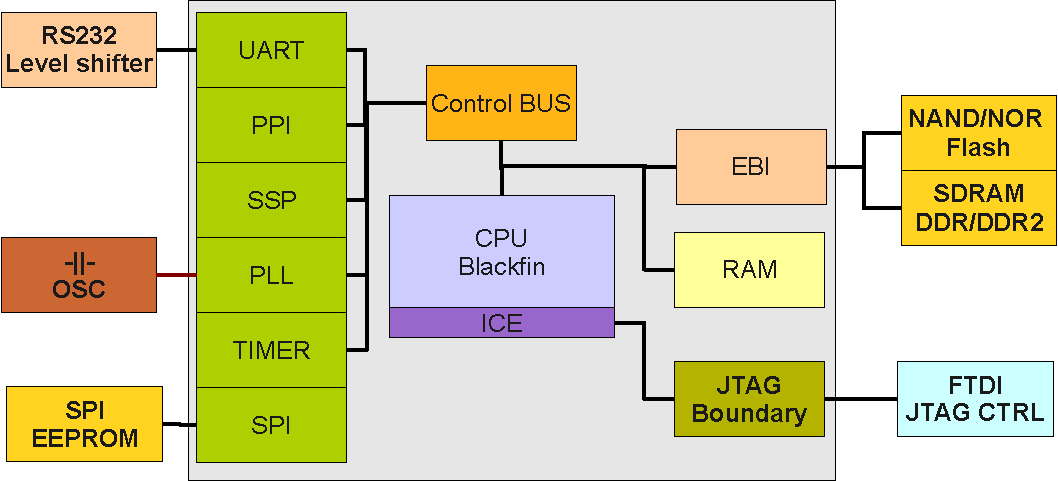
\includegraphics[scale=.32]{../images/ECB_BF532_Block.pdf} \\
       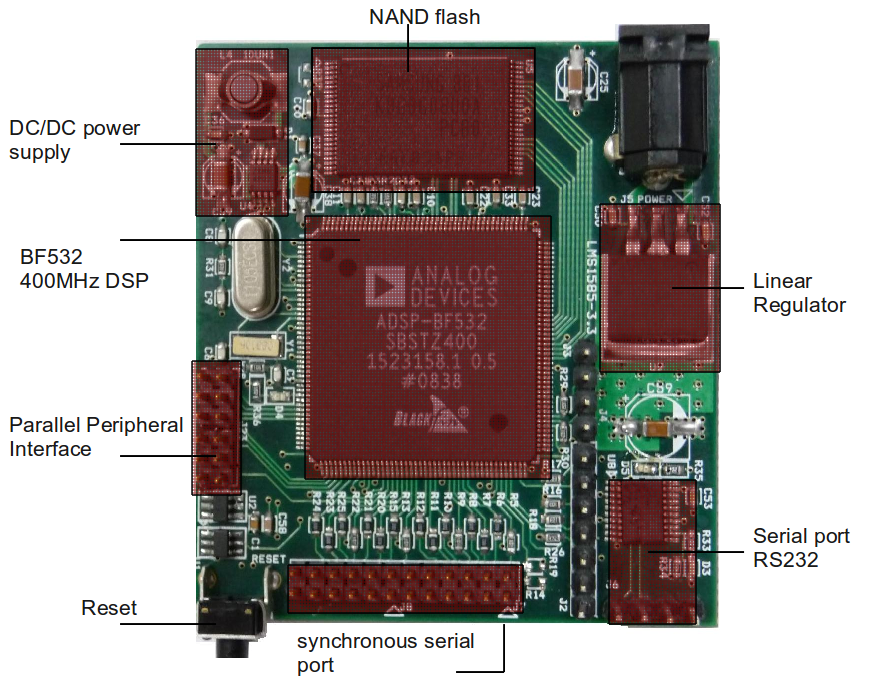
\includegraphics[scale=.18]{../images/ECB_BF532.png}
       \\
       \resizebox{!}{.4cm}{
          \footnotesize
          \begin{tabular}{|l|l|l|l|}
            \hline
            \textbf{CPU}  & \textbf{Capas} & \textbf{Montaje}  &\textbf{OS}
            \\ \hline
            Blackfin 400M &       4        & local Manual.     uCLinux
            \\ \hline 
          \end{tabular}
        }
    };
 
    \onslide<8> \node [ph_explain2, right=.5cm of adaptation.east] (exp_adaptation)    
    {
      \begin{center} \textbf{Plataforma SIE } \end{center}
      \centering
      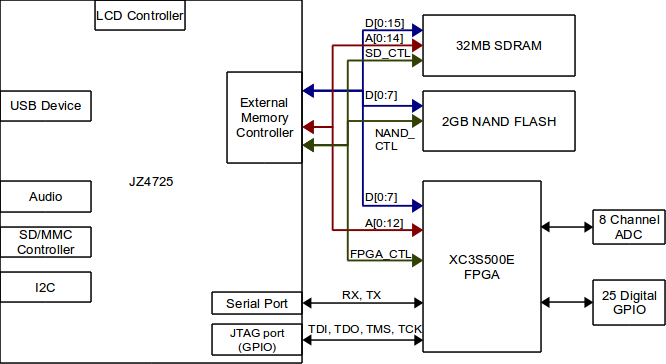
\includegraphics[scale=.35]{../images/SIE_block_diagram.png} \\
      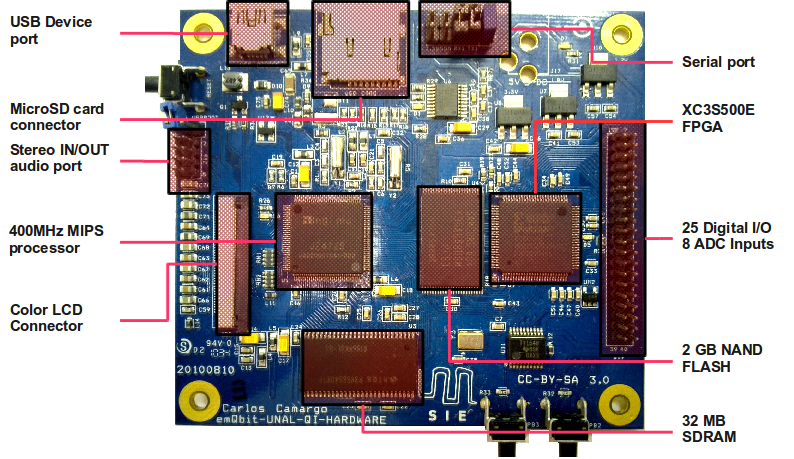
\includegraphics[scale=.2]{../images/SIE.jpg}
      \\
        \resizebox{!}{.4cm}{
            \footnotesize
            \begin{tabular}{|l|l|l|l|}
              \hline
              \textbf{CPU}  & \textbf{Capas} & \textbf{Montaje}  &\textbf{OS}
              \\ \hline
              ARM7,50M     &    2           & local Manual.     & eCos
              \\ \hline 
            \end{tabular}
        }
    };


    \onslide<9> \node [ph_explain2, right=.5cm of adaptation.east] (exp_adaptation)    
    {
      \begin{center} \textbf{Plataforma STAMP } \end{center}
      \centering
      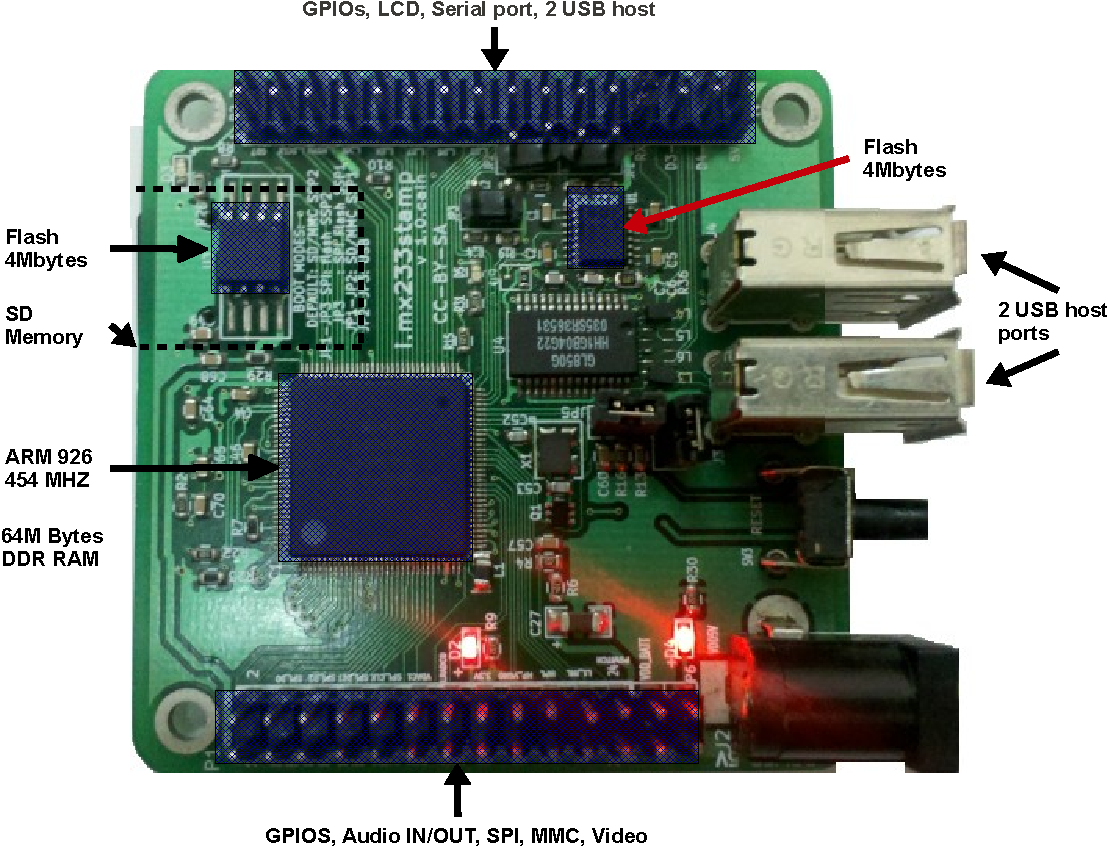
\includegraphics[scale=.3]{../images/stamp_block.pdf}
      \\
        \resizebox{!}{.4cm}{
            \footnotesize
            \begin{tabular}{|l|l|l|l|}
              \hline
              \textbf{CPU}  & \textbf{Capas} & \textbf{Montaje}  &\textbf{OS}
              \\ \hline
              ARM 926 400M  &      2         &  Local Manual     & Linux, Android 
              \\ \hline 
            \end{tabular}
        }
    };

    \onslide<10> \node [ph_explain2, right=.5cm of adaptation.east] (exp_adaptation)    
    {
      \begin{center} \textbf{ Res�men plataformas } \end{center}
      \centering
        \resizebox{!}{1.5cm}{
            \footnotesize
            \begin{tabular}{|l|l|l|}
              \hline
              \textbf{Plataforma} & \textbf{Cant.}  &\textbf{Usuario}
              \\ \hline 
              ECB\_ARM7         & 2       & UN
              \\ \hline 
              UN\_UIS\_XPORT    & 2       & UN, UIS
              \\ \hline 
              ECB\_AT91\_V1     & 100     & UN, UIS, ULA, ENAP, UDFJC, USTA
              \\ \hline 
              ECB\_AT91\_V2     & 30      & UN, UIS, ULA, ENAP, UDFJC 
              \\ \hline 
              ECBOT             & 20      & UN, UIS
              \\ \hline 
              ECB\_BF532        & 5       & UN
              \\ \hline 
              SIE               & 150     & UN, UIS, ULA, ECI
              \\ \hline 
              STAMP             & 10      & UN, ULS, 
              \\ \hline 
            \end{tabular}
     }
     
    };
   


    \onslide<11> \node [ph_explain2, right=.5cm of adaptation.east] (exp_adaptation)    
    {

      \begin{center} \textbf{Proceso de Fabricaci�n de PCBs} \end{center}
      \centering
      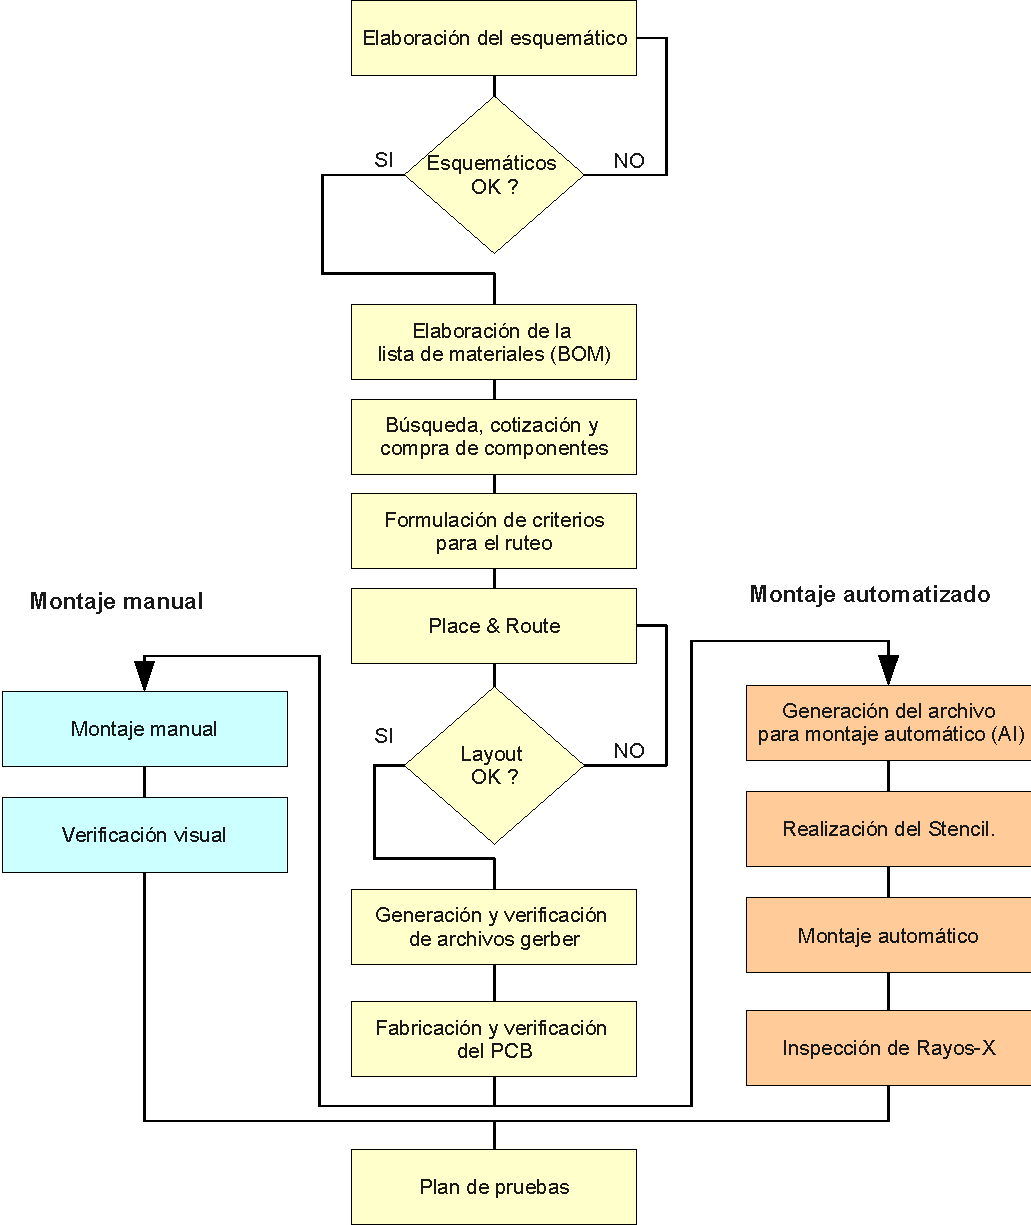
\includegraphics[scale=.41]{../images/proceso_de_fabricacion_PCBs.pdf}
    };

    \onslide<12> \node [ph_explain2, right=.5cm of adaptation.east] (exp_adaptation)    
    {
      \begin{center} \textbf{Flujo de ingenier�a inversa} \end{center}
      \centering
      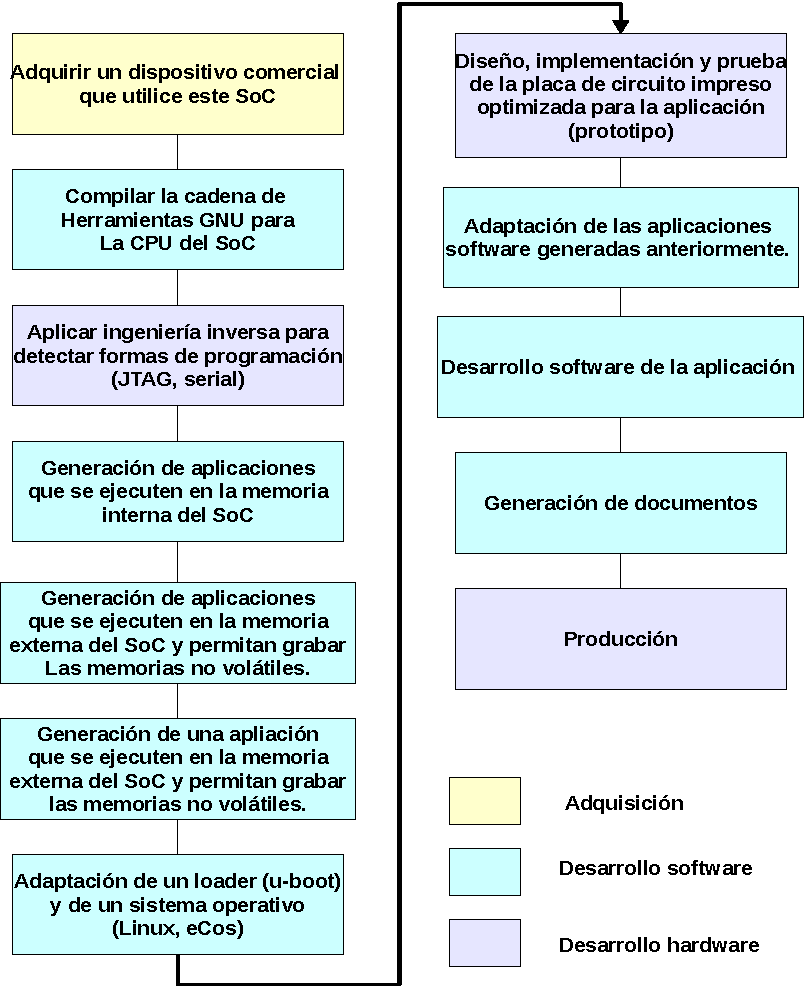
\includegraphics[scale=.47]{../images/SoC_reverse.pdf}
   };
 
\end{tikzpicture}
\end{figure}

\end{frame}